\begin{figure}[t]
\centering
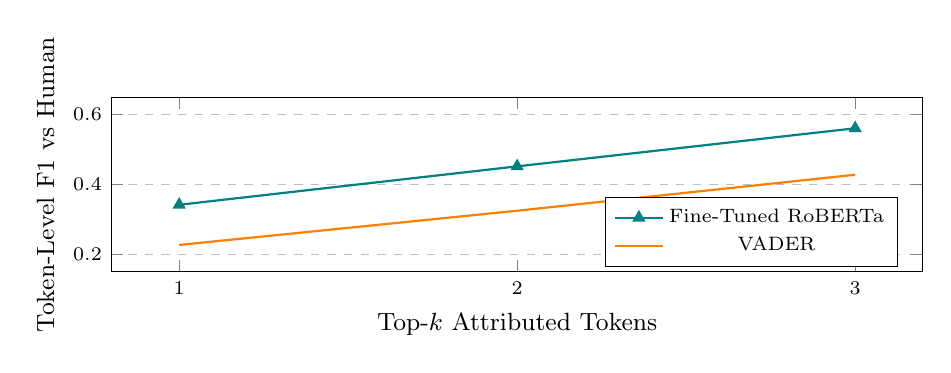
\begin{tikzpicture}
\begin{axis}[
    width=0.98\columnwidth,
    height=3.8cm,
    xlabel={Top-$k$ Attributed Tokens},
    ylabel={Token-Level F1 vs Human},
    xmin=0.8, xmax=3.2,
    ymin=0.15, ymax=0.65,
    xtick={1,2,3},
    legend pos=south east,
    legend style={font=\scriptsize},
    label style={font=\small},
    tick label style={font=\scriptsize},
    ymajorgrids=true,
    grid style=dashed,
    every axis plot/.append style={thick}
]
\addplot[color=teal,mark=triangle*] coordinates {
    (1, 0.342) (2, 0.452) (3, 0.561)
};
\addlegendentry{Fine-Tuned RoBERTa}
\addplot[color=orange,mark=circle*] coordinates {
    (1, 0.227) (2, 0.325) (3, 0.428)
};
\addlegendentry{VADER}
\end{axis}
\end{tikzpicture}
\caption{Plausibility F1 Progression across Top-$k$ feature attributions against 100 human-annotated headline rationales.}
\label{fig:plausibility}
\end{figure}